\section{Discussion}
\label{sec:discussions}

%==============================================================================
\subsection{The Goldilocks Model and Polarization}

The fiducial models cover a regular grid in parameter space.
In one instance, for \kharma models, adjacent points in parameter space fail only one constraint for opposite reasons: the SANE, $\abh = 0.5$, $\Rh = 40$ $i = 10\degree$ models fails because the 86\GHz image is too small, while the $i = 30$deg models fail because the 86\GHz image is too large, suggesting  that a model with intermediate inclination would pass all constraints.

We analyzed a representative, intermediate inclination \kharma SANE model with $i = 20\degree$.
This ``goldilocks'' model passes {\em all} constraints (we did not compute the X-ray luminosity but the $i=10$ and $i=30\degree$ models pass).

We have imaged a series of \kharma models with inclinations between $10$ and $30\degree$.
The cause of the inclination sensitivity is an extended, 86\GHz-bright, jet.
At $i = 10\degree$ the jet is nearly parallel to the line of sight and the source size is dominated by the accretion flow, but as $i$ increases the jet, which is radially extended, begins to extend past the accretion flow and dominate the source size.

Despite this success we regard the goldilocks model as unpromising for two reasons.
First, the $10$ and $30\degree$ \bhac models fail the X-ray constraint, and the neighboring $10$ and $50\degree$ \hamr models fail several constraints.

In addition, the goldilocks model is likely underpolarized at 230\GHz.
The source-integrated linear polarization of \sgra at the time of the 2017 campaign was between $6.9$ and $7.5$\% \citep{2021ApJ...910L..14G}, and this is consistent with historical measurements.
We will consider linear and circular polarizations in future papers, but the preliminary result is that the goldilocks model has linear polarization $\approx 1$\%, which would fail the goldilocks model.
The best-bet region MAD models, considered below, have linear polarization comparable to that observed.

%==============================================================================
\subsection{Testing Exploratory Models that Pass}

Six exploratory models, considered in Section \ref{sec:explore},  pass all constraints.
Although they appear promising these six models are imaged for only $5,000 \tg$ and thus  have been tested more weakly than the fiducial thermal models.

We imaged each of the passing exploratory models on to $15,000 \tg$.
All failed one or more constraints, and these are listed in Table \ref{tab:fail_none}.
Evidently the exploratory models, and particularly the models with nonthermal electrons, do not provide any models that pass all constraints.

We draw two conclusions from this.
First, the pass/fail status of the model can be sensitive to the length of integration, and it is important to image the models for at least $15,000\tg$.
In connection with this we note that the \koral models, which were imaged at 230\GHz for $\sim 10^5 \tg$, were generally consistent with the fiducial models but provide tighter $\mi{3}$ constraints (see Appendix \ref{app:variability}).
Second, the constraints that are most sensitive to model duration are $\mi{3}$ (all models failed $\mi{3}$ after being extended) and the \mring fits (two failed \mring width, one failed \mring diameter).

%==============================================================================
\subsection{Origin of Variability Excess}

Approximately 84\% (\kharma), 73\% (\bhac), and 97\% (\hamr) of the fiducial models fail one or both variability constraints.
This naturally leads one to ask whether there is an observational or modeling problem with these constraints.

For example, it is possible that a fraction $f_\mathrm{ext}$ of the $230\GHz$ flux density is in an extended structure (e.g. a jet) that is slowly varying, unresolved by ALMA, and resolved out by EHT.
The observed $\mi{3}$ would then be smaller than the true $\mi{3}$ for the compact source by a factor of $1/(1 + f_\mathrm{ext})$.
The $4$G$\lambda$ amplitude variability is normalized by the lightcurve and thus $a_4$ would be suppressed by a similar factor.

Diffuse emission on scales larger than the VLBI images ($\sim 100\uas$) and smaller than connected element interferometer measurements ($\sim 100\,\mathrm{mas}$) is difficult to constrain.
The EHTC imaging strategy involves a self-calibration step that assumes no diffuse structure on scales between the zero-baseline and the shortest VLBI baselines (\citetalias{PaperIII}).
However, longer wavelength VLBI observations place constraints on any emission on these scales under the assumption of flat or steep spectra.
For instance, $230$ and $43\GHz$ VLBI observations that use the Los Alamos-Pie Town-VLA baselines probe scales of $\sim 1$ to $10\,\mathrm{mas}$ and demonstrate no inconsistency in closure amplitudes and closure phases with a symmetric, two-dimensional Gaussian model \citep{2004Sci...304..704B}.
VLBI observations at 3mm wavelength are also fully consistent with a two-dimensional Gaussian model with an upper limit of $\sim 10\,\mathrm{mJy}$, or approximately 1\% of the total flux density \citep{2019A&A...621A.119B}.
Additionally, a dust contribution is constrained by shorter wavelength ALMA observations that find a flat or slightly falling spectrum up to 900 GHz \citep{2019ApJ...881L...2B}.
A substantial diffuse dust contribution would only be consistent if its properties were tuned to match a steeply falling compact synchrotron spectrum, which would likely be inconsistent with the substantially variable far infrared component of \sgra emission \citep{2016ApJ...825...32S, 2018ApJ...862..129V}.

Future observations with short-baseline coverage such as that provided by the Kitt Peak to SMT baseline will enable tighter constraints on any diffuse component.
If confirmed, the presence of diffuse flux would require re-normalization of the models and re-evaluation of the constraints.
A reduction of $\sim 30\%$ in the compact flux would lead many SANE models to fail the \mi{3} constraint because they would be not variable enough and would lead most MAD models to pass the \mi{3} constraint.
Since $F_{230} \sim \dot{M}^2$ a $15\%$ change in model density normalization, and therefore in optical depth, would suffice.

The variability excess might also be caused by physical incompleteness of the models.
Collisionless effects and radiative cooling could both reduce variability.

We model the accreting plasma as an ideal fluid when in fact it is collisionless, with Coulomb mean free path large compared to $\rg$.
This is less worrisome than one might think: electrons and ions are confined to helical orbits around field lines, implying an effective mean free path perpendicular to the field lines of order the gyroradius $\sim 56 \Theta_e [B/(30\,\mathrm{G})]^{-1} \cm \ll \rg$.
The mean free path parallel to field lines is still long, but may be governed by scattering off electromagnetic field fluctuations excited by kinetic instabilities rather than Coulomb scattering.

Future global kinetic general relativistic particle-in-cell simulations may be able to test how well the ideal fluid model describes collisionless accretion flows.
Meanwhile, a relativistic fluid model incorporating small collisionless corrections was developed by \citet{2015ApJ...810..162C} and studied numerically by \citet{2017MNRAS.470.2240F}.
The leading order corrections are conduction and pressure anisotropy (i.e. viscosity).
The effect of conduction and viscosity on our constraints is not known, but it is known that viscosity reduces turbulent stress in SANE models \citep{2017MNRAS.470.2240F}, consistent with a reduction in variability.
It is also plausible that conduction smoothes out temperature maxima, possibly also leading to a reduction in variability.

Our models also neglect radiative cooling.
Cooling is fastest where the electron temperature is highest, so cooling has the potential to blunt  local maxima in temperature.
If local maxima with short cooling times contribute significantly to variability then cooling could reduce $\mi{3}$.
Self-consistent cooling requires integration of an electron energy equation  \citep[e.g.]{2015MNRAS.454.1848R}, and assignment of a density scale (mass unit or accretion rate) when the GRMHD simulation is run, vastly increasing computational cost.

Another possibility is that self-consistent electron heating reduces variability.
In Appendix \ref{app:variability} we consider a set of models from \citet{2020MNRAS.494.4168D}
with self-consistent electron heating.
These models show similar variability excess to the $\Rh$ models.

The $\Rh$ prescription contains a parameter $\Rl$ that determines the ion-electron temperature ratio at low $\beta$, which we have consistently set to $1$.
Increasing $\Rl$ models the effect of rapid cooling in low $\beta$ regions.
In Appendix \ref{app:variability} we consider $\Rl$ up to 10 in a sample of four models and show that it does not systematically reduce variability.

The variability excess might also be caused by: numerical inaccuracies in radiative transfer, truncation error in the GRMHD integrations (limited resolution), limited simulation duration, or misspecification of the adiabatic index.
These are considered in Appendix~\ref{app:numerical}.
We find no evidence that any of these numerical effects is driving the variability excess.

%==============================================================================
\subsection{Best-Bet Region without Variability}

From the preceding discussion it is possible that a  combination of extended flux, viscosity, cooling, and numerical limitations affect model variability enough to compromise the variability constraints.
Notice that a relatively small change in variability, $\sim$ 30\% in \mi{3}, is sufficient to promote many of the MAD models from failing to passing.
If we exclude the variability constraints, then, which models are favored?

\begin{figure*}
  \centering
  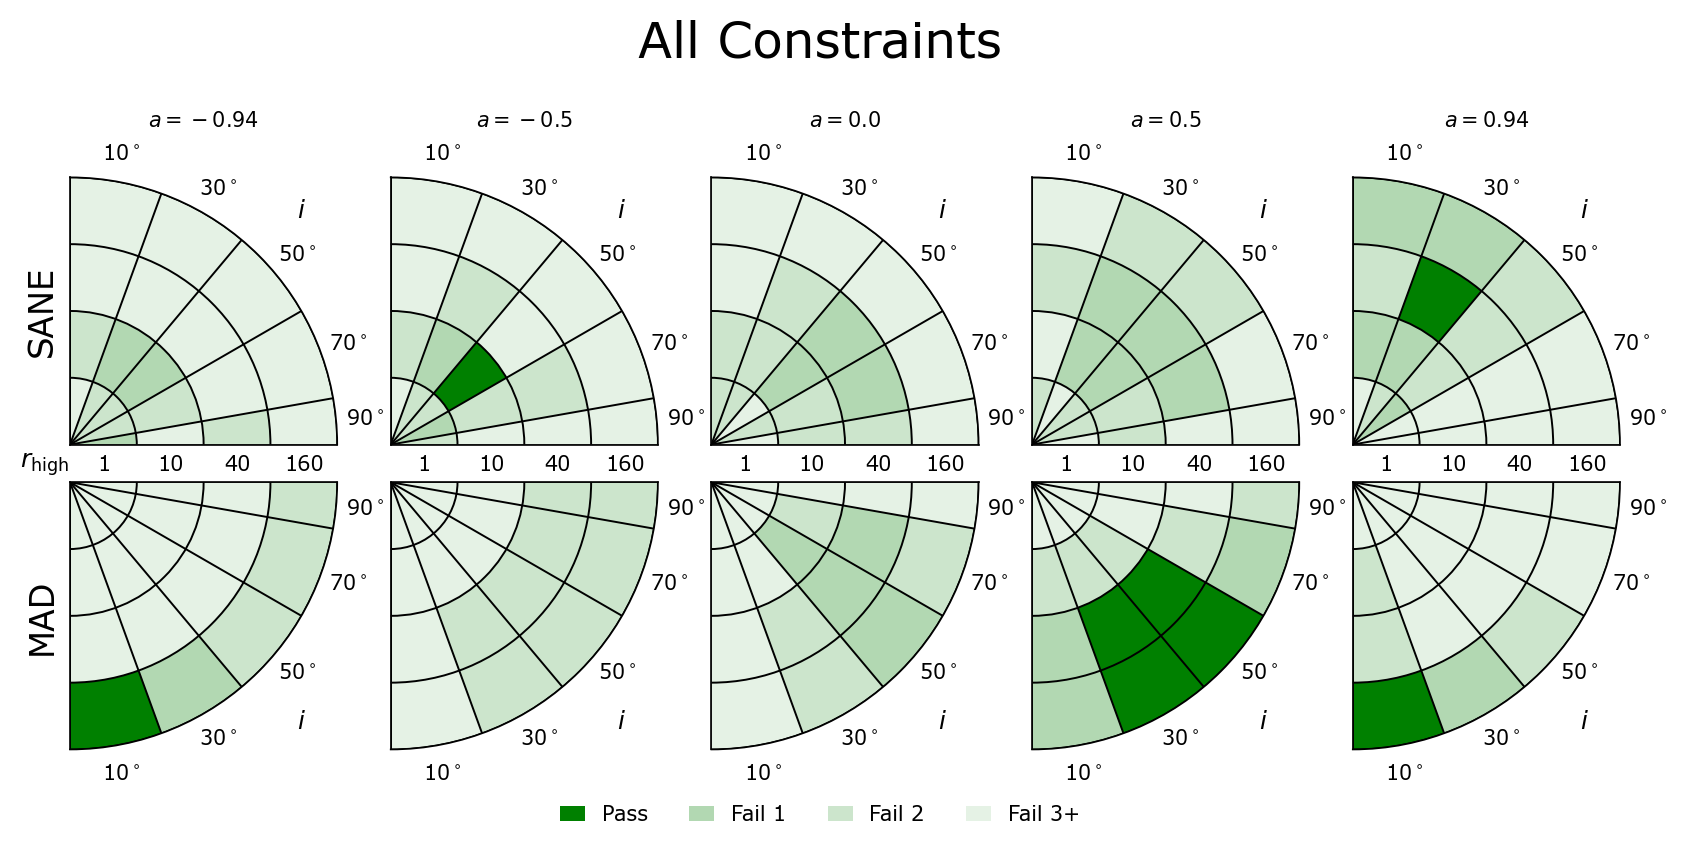
\includegraphics[width=0.8\textwidth]{./figures/All_Constraints.png}
  \caption{Combined constraints without structural or flux variability.
Green indicates that the \kharma, \bhac, and (for $i = 10, 50, 90$deg) \hamr models pass, yellow that one or two of the fiducial models fail, and red that all models fail.}
  \label{fig:all_pizza}
\end{figure*}

Figure~\ref{fig:all_pizza} (which is also repeated in Figure~\ref{fig:all_pizza_app} in the appendix) shows the result of applying all constraints except structural and flux variability to the fiducial models.
Most negative spin models are ruled out, and three MAD, positive spin, low inclination, large $\Rh$ models pass all constraints for \kharma, \bhac, and (at $i = 10$deg) \hamr.
Nearby models in parameter space are close to passing in the sense that they pass for one or more of \kharma, \bhac, and \hamr.

We will call the green region of parameter space in Figure \ref{fig:all_pizza} the {\em best-bet region}.
The models in this part of parameter space perform well and explain nearly all the data.

Given the uncertainty associated with the variability excess and the possibility of missing physical ingredients in the model the existence of the best-bet region cannot be regarded as evidence that \sgra has positive spin and low inclination.
It is remarkable, however, that {\em any} models perform as well as these do.
The models in the best-bet region merit additional analysis, and it is interesting to ask what they predict for future observations.

%==============================================================================
\subsection{Fiducial Models Accretion Rate and Outflow Power}
\label{sec:accrate_outflowpower}

\begin{figure*}
  \centering
  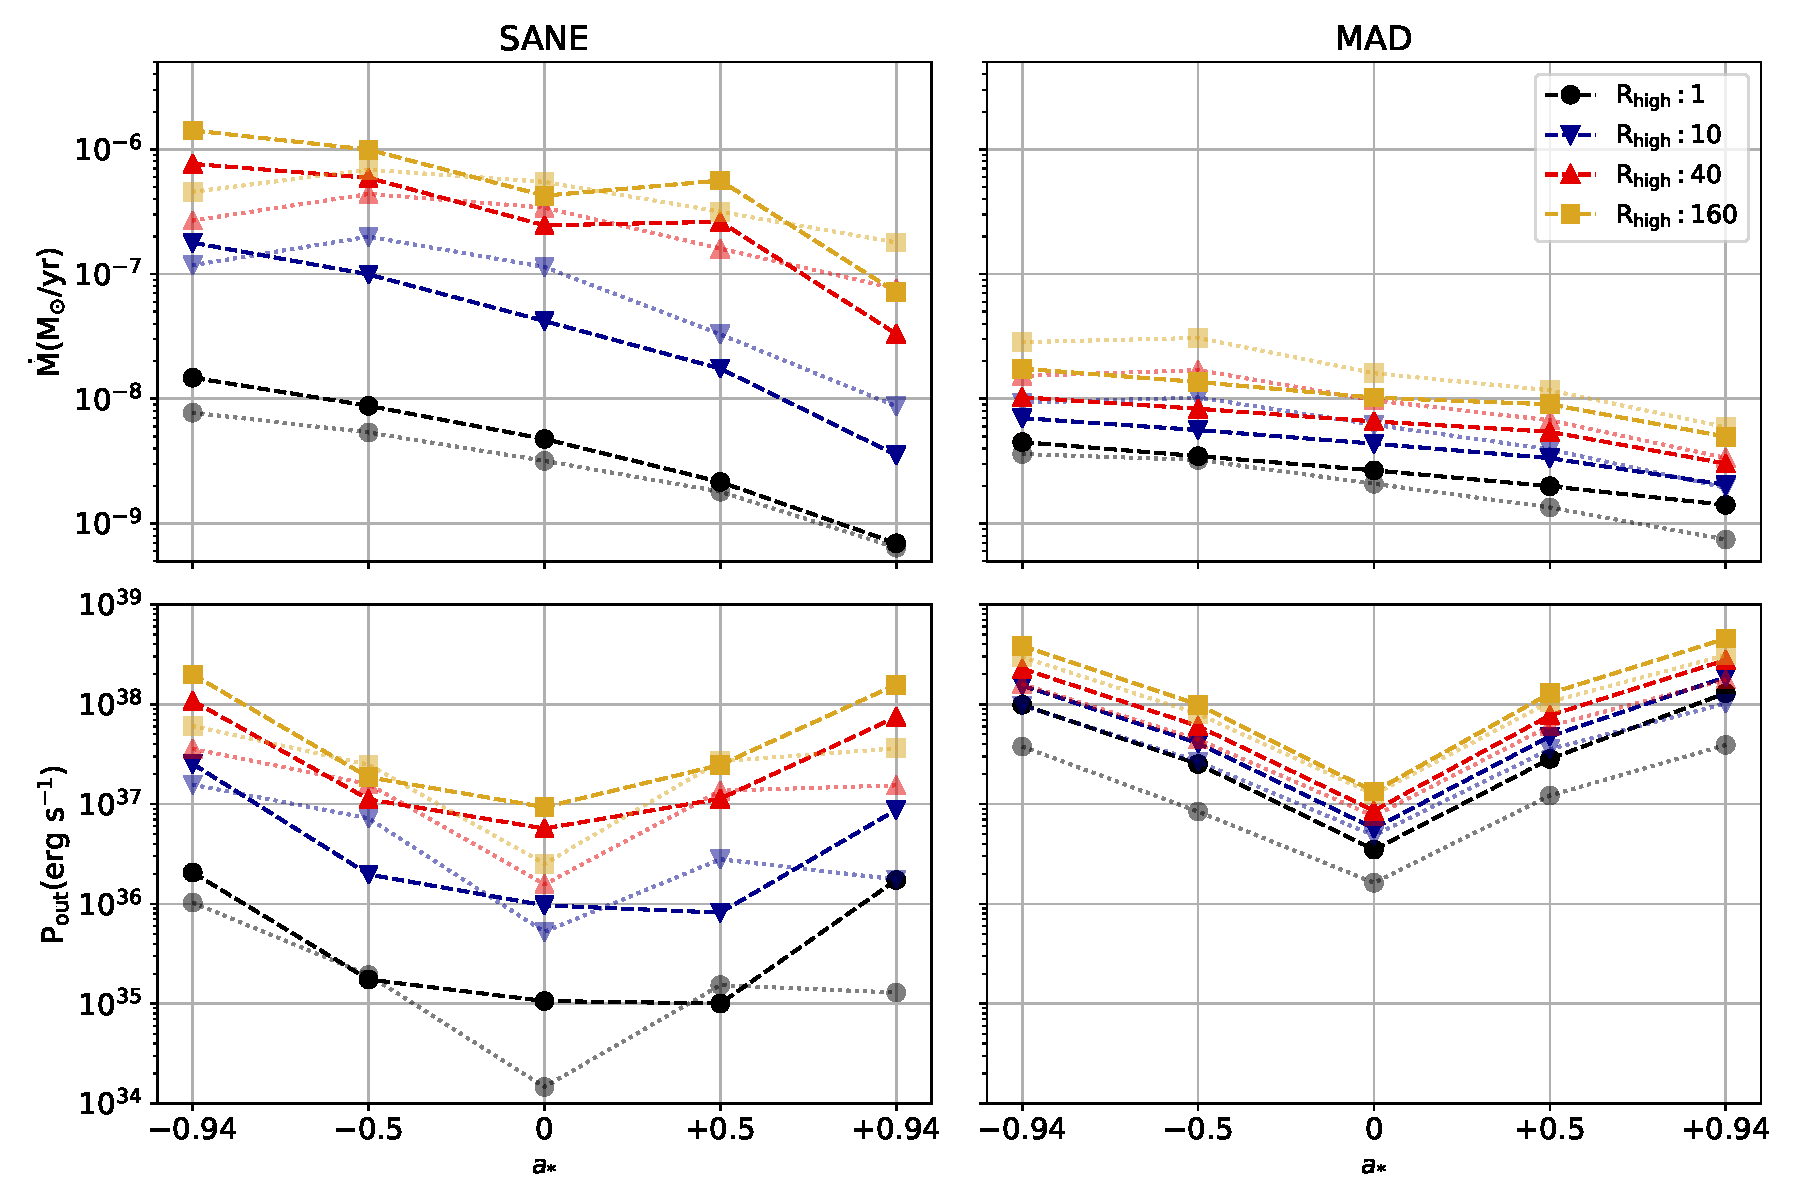
\includegraphics[width=0.95\textwidth]{figures/bhac_kharma_average_mdot_pout.pdf}
  \caption{{\it Top:} Accretion rate $\dot{M}$ for standard models.
    Since $\dot{M}$ depends weakly on inclination $i$, we show only $i=50\degree$.
    {\it Bottom:} Outflow power $P_\mathrm{out}$ for standard models at $i = 50\degree$.
    The colors and markers vary with $\Rh$.
    The dashed lines correspond to \kharma thermal models while the dotted lines indicate \bhac thermal models.}
  \label{fig:accretion_outflow_power_illinois_thermal}
\end{figure*}

What is the accretion rate in \sgra?  In our models, we measure the time-averaged accretion rate
\begin{equation}
  \dot{M} = \frac{1}{\Delta t}\int dt\int d\theta d\phi\hspace{0.1cm}\sqrt{-g}\big(-\rho u^{r}\big),
\end{equation}
at the event horizon; the quantity in the parenthesis is the inward rest-mass flux.

Figure~\ref{fig:accretion_outflow_power_illinois_thermal} (top panels) shows the time-averaged $\dot{M}$ (in solar masses per year) for the \kharma and \bhac thermal models.
The accretion rates follow immediately once the models are normalized so that $\langle F_{230}\rangle = 2.4\,\mathrm{Jy}$.
A listing of $\dot{M}$ for all models for which it is available is provided in Appendix \ref{app:tables}.

The MAD models accrete at $10^{-9}$ to $10^{-8} M_{\odot}$yr$^{-1}$ while the SANE models have a broader range, $10^{-9}$ to $10^{-6} M_{\odot}$yr$^{-1}$.
$\dot{M}$ is an increasing function of $\Rh$.
This can be understood as a consequence of three facts: (a) the thermal synchrotron emissivity is an increasing function of temperature; (b) the electron temperature is inversely proportional to $\Rh$; (c) the models need to normalized so that $\langle F_{230}\rangle$ $=$ 2.4Jy.
The SANE models exhibit a stronger dependence on $\Rh$.
The emission in the SANE models is predominantly from regions with large $\beta$, where the electron temperature is regulated by $\Rh$.
MAD models produce a substantial fraction of the emission in regions with $\beta\sim 1$, where $\Rh$ does not notably influence electron temperature and thus have a weaker dependence on $\Rh$ (cite figure 4 in M87 paper V).
For both SANE and MAD models, $\dot{M}$ reduces with spin.
This follows from the dependence of temperature on spin shown in Figure 2: higher spin corresponds to higher temperatures

Retrograde SANE, $\Rh=40$ and $160$ models produce the largest accretion rates, $\dot{M} \sim 10^{-6}M_{\odot}\yr^{-1}$.
These models have a high midplane density of cool electrons that overproduce X-ray emission through bremsstrahlung and are therefore ruled out.
 Our critical beta models have accretion rates that lie between the standard model values for $\Rh = 10$ and $\Rh = 40$ for the selected critical beta parameter values ($f=0.5$, $\beta_\mathrm{crit}=1$).

How do our $\dot{M}$ compare with earlier estimates?  Linear polarization and Faraday rotation measurements at millimeter and sub-millimeter wavelengths \citep{2000ApJ...538L.121A, 2000ApJ...545..842Q, 2003ApJ...588..331B, 2006ApJ...640..308M, 2006JPhCS..54..354M, 2006ApJ...646L.111M} and X-ray emission \citep{2003ApJ...591..891B, doi:10.1126/science.1240755} combined  with semi-analytic models predict $\dot{M} \sim 10^{-9} - 10^{-7} M_{\odot}\yr^{-1}$.
The broad range of values is due to the differences in regions of radio emission in the theoretical models that are considered (ADAFs: \citealt{1998ApJ...492..554N, Yuan_2003}; Jet models: \citealt{1993A&A...278L...1F, 2000A&A...362..113F}; ADAF+jet models: \citealt{2002A&A...383..854Y}).
All our MAD $\dot{M}$ fall within the range of these historical observational estimates.
Interestingly almost all SANE models with larger $\rhigh$ parameter (except SANE $\abh=0.94$, which is one of our best models) have $\dot{M}$s that are inconsistent with earlier estimates.

All fiducial models produce outflows in the polar regions.
In many cases the outflows can be divided into a slower, denser disk wind and a relativistic, high $\sigma$ Poynting jet.
The outflows have a power that is comparable to or larger than the bolometric luminosity.
What is the outflow power $P_\mathrm{out}$?

First we must define $P_\mathrm{out}$.
There are a number of competing definitions in the literature: \citet{refId0}, \citet{2014A&A...570A...7M} cut on  Bernoulli parameter Be, while \citet{10.1111/j.1365-2966.2012.22002.x} consider the ratio of energy flux to rest mass flux $\mu$, and \citetalias{M87PaperV} applies a $\beta\gamma$ cut to define $P_\mathrm{out}$.
Here we use the time-averaged outflow power near the poles \citepalias{M87PaperV}:
\begin{equation}
  P_\mathrm{out} \equiv \frac{1}{\Delta t}\int dt \int d\phi \int_\mathrm{poles} d\theta \sqrt{-g}\left(-T^{r}_{t}-\rho u^{r}\right),
\end{equation}
where ``poles'' means $\theta < 1\,\mathrm{rad}$ or $\theta > (\pi-1)\,\mathrm{rad}$ at those $\theta$ where the time- and azimuth-averaged energy flux is outward.
The integral is evaluated at $r = 100\rg$.
$P_\mathrm{out}$ includes power in the relativistic Poynting jet, if present, and in the slower, denser disk wind.

In Figure~\ref{fig:accretion_outflow_power_illinois_thermal}
(bottom panels) we compute $P_\mathrm{out}$ for the standard models.
As expected, the outflow power increases with black hole spin magnitude.
SANE models have $P_{out}$ in the range ~$10^{35} \ergps$ to $10^{38} \ergps$.
Evidently $P_{out}$ increases with $\Rh$,  reflecting the behavior of $\dot{M}$: higher $\dot{M}$ models have stronger magnetic fields.
MAD models have $P_\mathrm{out}$ in the range $10^{37}$--$10^{39} \ergps$ and are, on average, larger and less sensitive to $\Rh$, again reflecting the behavior of $\dot{M}$.

Many high spin or large $\Rh$ models have $P_\mathrm{out} \sim 10^{38} \ergps$.
An outflow with this power could produce dramatic observable effects in the dense interstellar medium of the Galactic Center.
For instance, the X-ray transient CXOGC J174540.0-290031, located only 0.1\pc from \sgra and with an estimated jet power of $\sim 10^{36}\ergps$ produced a compact bipolar lobe at radio wavelengths with peak flux densities near 100$\,\mathrm{mJy}$ \citep{2005ApJ...633..218B}.
A more continuous  outflow, however, might clear out a substantial volume of space, making identification of any interaction with the ISM less certain.
Nevertheless, there have been a number of large scale features that have been suggested as the result of interaction of a jet with the ISM \citep[e.g.,][]{2013ApJ...779..154L,2021ApJ...922..254C}.

%==============================================================================
\subsection{Electron Distribution Function}

One of the central uncertainties in modeling \sgra is electron distribution function (eDF) assignment.
Do the surviving models have anything to say about the eDF?

In our standard models, thermal eDFs with equal ion and electron temperature ($\Rh = 1$) are ruled out, in most cases by more than one constraint.
For MAD models this is easily explained: Comptonization is strong at $\Rh = 1$ and X-rays are overproduced.
The electron temperature is a maximum when $\Rh = 1$, if all other parameters are fixed.
For MAD models, $\dot{M}$ and therefore the electron scattering optical depth $\tau_\mathrm{es}$ is insensitive to $\Rh$.
Since the amplitude of the first Compton bump is $\propto y = 16 \Theta_e^2 \tau_\mathrm{es}$, the high $\Theta_e$ at $\Rh = 1$ produces a large X-ray flux.
For SANE models the situation is more complicated (see Appendix~\ref{app:tables}), with an \mring width rejecting many $\Rh = 1$ models at $\abh \le 0$, and 86~GHz flux and size rejecting the rest.
The latter is a consequence of model electron temperature reaching a maximum at large $\abh$ and low $\Rh$, so that optical depth is minimum and therefore so is the 86~GHz image size.

In standard SANE models the sense of the X-ray constraint is reversed: bremsstrahlung is strong and X-rays are overproduced where $\Rh$ is {\em large}.
Again this is easily understood: when $\Rh$ is large the midplane electrons are cold, the accretion rates (and therefore $n^2$) are high, and the bremsstrahlung emissivity is large.
More generally the X-rays provide a strong constraint on the presence of dark (subrelativistic) electrons, which are otherwise undetectable in millimeter wavelength emission or absorption, although they can produce strong Faraday rotation.

We have also tested a large set of nonthermal models, which have a power-law tail on the eDF.
Although integration times for the nonthermal models are too short to provide strong model constraints, there are trends that emerge from the existing data.

First, the 230~GHz images are relatively insensitive to the presence of nonthermal electrons, at least for the nonthermal electron models we have studied here.
This is encouraging: the 230~GHz image is generated by electrons in an approximately thermal core of the eDF, and is relatively insensitive to the behavior of the tails.

Second, as one might expect, the 2.2\um flux density is a strictly increasing function of nonthermal electron density.
In many models (e.g.
the variable efficiency models of Section 4.2.3) the addition of a power-law tail changes a thermal model that passes the $2.2\um$ test into a nonthermal model that fails.

Third, it is important to understand that many of the nonthermal models we use are linked to the $\Rh$ prescription in some way.
For example, the $\kappa$ distribution function contains a width parameter $w$, and this is set using an $\Rh$-like prescription with width depending on $\beta$.
Our nonthermal models are only a few points in a vast function space of possible nonthermal parameterizations, with none of the models considered allowing for an electron energy density that depends on plasma history as well as instantaneous plasma state.

%==============================================================================
\subsection{Caveats and Limitations}\label{sec:limits}

%------------------------------------------------------------------------------
\subsubsection{Collisionless plasma effects}

{The mean free path to Coulomb scattering for particles is typically larger than or comparable to the system size in \sgra, rendering its plasma collisionless.
The GRMHD simulations used in this work describe a collisional system, whereas a first-principles modeling of the collisionless plasma requires a fully kinetic treatment.
General relativistic (radiative) kinetic simulations are crucial for dynamically probing the electron temperature, effects of non-thermal distribution functions, and pressure anisotropy and their interplay with radiation in collisionless plasma in the accretion disk and jet.
While global general relativistic kinetic simulations cannot be performed with full physical separation between microscopic plasma scales (the particle's Larmor radius $r_{\rm L}$, and plasma skin depth $d_{\rm e}$) and macroscopic scales (the gravitational radius $r_{\rm g}$), they can achieve the right hierarchy of scales ($r_{\rm g} \gg d_{\rm e} \gg r_{\rm L}$) for magnetized plasmas \citep{2018A&A...616A.184L,2018ApJ...863L..31C,2019PhRvL.122c5101P,2020PhRvL.124n5101C,2020ApJ...895..121C,2020ApJ...902...80K,2021A&A...650A.163C,2021PhRvL.127e5101B}.
Even in GRMHD, it is computationally challenging to resolve plasma heating processes powering the observed radiation in a converged manner.
It is currently not yet feasible to resolve dissipation at the smallest scales of the turbulent cascade or the interplay between turbulence and reconnection at a similar level as in local box simulations \citep{2012ApJ...755...50R,2013ApJ...773..118H,2015PhRvL.114f1101H,2016PhRvL.117w5101K,2017PhRvL.118e5103Z,2018PhRvL.121y5101C,2018ApJ...859..149I,2019PhRvL.122e5101Z,2021ApJ...921...87N,2021ApJ...923L..13C}.
However, \citet{2019ApJS..243...26P} and \citet[in prep.]{Olivares_et_al} show that the global accretion dynamics (mass accretion rate, magnetic flux on the horizon, and MRI quality factor) are converging between the different simulations in this work.
Kinetic processes in the (near-)collisionless plasma may increase the effective particle collision rate \citep[see, e.g.,][]{2016PhRvL.117w5101K}.
Deviations from the infinitely conductive ideal fluid approximation may alter the thermodynamics of the flow \citep[see, e.g., ][and Appendix C1]{2017MNRAS.470.2240F}.
Some aspects of (near-)collisionless plasma dynamics can be described with non-ideal effects (e.g., viscosity, resistivity, heat conduction, pressure anisotropy) in GRMHD simulations of black hole accretion, e.g.,  \cite{2014MNRAS.440L..41B,2015ApJ...810..162C,2016MNRAS.456.1332F,2017ApJ...837...92C,2017MNRAS.470.2240F,2018ApJ...859...28Q,2019ApJS..244...10R,2019ApJ...882....2V,2020ApJ...900..100R,2021PhRvD.104j3028M,2021arXiv211103689N,2021arXiv211105752M}.
For example, the first efforts have recently been made with high-resolution global GRMHD simulations to capture heating through magnetic reconnection in the largest current sheets in the system \citep{2020MNRAS.495.1549N,2020ApJ...900..100R,2021MNRAS.508.1241C,2022ApJ...924L..32R,2021arXiv211103689N}.}

%------------------------------------------------------------------------------
\subsubsection{Positrons}\label{sec:pair}

So far we have considered only ion-electron plasmas, but pairs can be produced in the 230 GHz emission region through pair discharges or through so-called pair drizzle.
How might our neglect of pairs affect the models?

The importance of pairs has been assessed using phenomenological models \citep{2020ApJ...896...30A, 2021ApJ...923..272E} and depends sensitively on the efficiency with which a reservoir of magnetic energy can be converted into pairs.
If this efficiency is large then pairs can substantially increase intensity in the jet region.

Production of pairs through the drizzle process is weak in \sgra because its luminosity is so low.
\cite[][see also \citealt{2021ApJ...907...73W}]{2011ApJ...735....9M} estimate the drizzle pair density of \sgra to be $10^{-8}\cm^{-3}$.
This is well below the Goldreich-Julian density $\sim \abh B c^2/(4 \pi e G M) \sim 10^{-2} \abh [B/(30 {\rm G})] \cm^{-3}$ required to screen electric fields, suggesting pair discharges are likely.
If pair discharges serve only to raise the pair density to the Goldreich-Julian density, however, then the jet is unlikely to outshine the accretion flow, where the magnetic field strength is similar to that in the jet but the characteristic number density is $\sim 10^6 \cm^{-3}$.
The maximum conceivable impact of pairs on EHT observations is obtained by converting about half of the magnetic energy density into pairs with Lorentz factor $\sim 30$ so that in \sgra's $\sim 30$G magnetic field the emissivity of the resulting pairs peaks close to 230\GHz.
Then the pair density $\sim 10^{6} \cm^{-3}$ and the jet might compete with the accretion flow.

%==============================================================================
\subsection{Outlook}\label{sec:future}

Except for the brief discussion above, our analysis omits polarization.
Future analyses should test our models against integrated polarization of \sgra \citep{2021ApJ...910L..14G} and against polarized imaging, as was done for M87* \citepalias{M87PaperVII, M87PaperVIII}.

Our analysis also omits discussion of one of the main observational features of \sgra: the near infrared and X-ray flares, for which there is as yet no consensus model.
Our analysis is built on the notion that the near infrared flares, at least, could be produced by accelerating a small fraction of the electron population into a nonthermal tail.
The monotonic increase in $2.2\um$ flux density with nonthermal population seen in Section \ref{sec:comparisons} is consistent with this notion.

The agreement between our results on the source size and orientation and those of the GRAVITY collaboration \citep{2018A&A...618L..10G} also support the similarity in the spatial distribution of the electrons producing near-infrared flares and those responsible for the 230\GHz emission.
\citealt{2018A&A...618L..10G} find that the near-infrared flares originate from a region $\approx$ 40--50$\mu$as from the black hole, only slightly larger than the diameter of the \mring fit to the 230\GHz image.
Moreover, the combined results of our analysis point towards a low observer inclination, again consistent with the GRAVITY results of a hotspot orbiting at $\lesssim 40\degree$ from the plane of the sky.

For M87* we were able to identify a sense of rotation of the source from the asymmetry of the observed ring.
For \sgra we have not yet been able to identify a preferred position angle for the source or measure the amplitude of source asymmetry, perhaps because it is small (\citetalias{PaperIV}).
Current sparse baseline coverage sharply limits our ability to detect asymmetry, while future EHT campaigns will add new stations.
Unless the source is aligned and $i \approx 0$, all our models (which have a definite sense of rotation) predict that the brightest point on the ring is produced by Doppler boosting and should lie on the approaching side of the accretion flow.
The sense of rotation could then be compared to the clockwise motion of near infrared flares observed by GRAVITY \citep{2018A&A...618L..10G}.

Our analysis shows the value of simultaneous measurements.
Simultaneous or near-simultaneous GMVA observations, in particular, provide a powerful constraint on the models.
The eDF is a major source of uncertainty in our analysis, and since the submillimeter (submm) and 2.2\um flux density are most sensitive to the eDF, future analyses should incorporate submm data and future EHT campaigns should seek simultaneous observations.

Our analysis provides some guidance for future numerical modeling of \sgra.
It is clear that models require long integrations ($\gtrsim  30,000 \tg$) to provide a converged characterization of the source.
We also note that there are regions in parameter space where we may not have sampled densely enough---where, for example, the model is too large and too small at adjacent points in parameter space.
An example of this is the 86GHz size measurement, which is sensitive to inclination, as seen for the goldilocks model.
We found that being able to compare three simulation pipelines helped us identify numerical sensitivities and saved us from errors on a number of occasions.
One point raised in these comparisons is that the $2.2\um$ flux density is sensitive to where emission is cut off in high $\sigma$ regions of the flow---the so-called $\sigma_\mathrm{cut}$ parameter.
This point merits future investigation.

Throughout this work we have assumed that the mass and distance to \sgra are known.
This assumption could be relaxed and the models checked for consistency with the stellar orbit measurements of mass and distance.
Phenomenological accretion flow models are particularly well suited to this type of study where the number of parameters is large  \citep[e.g.,]{2009ApJ...697...45B}.
